% TODO png blur? too wide listings
\chapter{Analyzing unknown binary files using information entropy}
\label{entropy}
\myindex{Entropy}

(This part has been first appeared in my blog at 13-May-2015.
Some discussion: \url{https://news.ycombinator.com/item?id=9545276}.)

For the sake of simplification, I would say, information entropy is a measure, how tightly some piece of data can be compressed.
For example, it is usually not possible to compress already compressed archive file, so it has high entropy.
On the other hand, one megabyte of zero bytes can be compressed to a tiny output file.
Indeed, in plain English language, one million of zeroes can be described just as ``resulting file is one million zero bytes''.
Compressed files are usually a list of instructions to decompressor, like this: ``put 1000 zeroes, then 0x23 byte, then 0x45 byte, then put a block of size 10 bytes which we've seen 500 bytes back, etc''.

Texts written in natural languages are also can be compressed tightly, 
because natural languages has a lot of redundancy
(otherwise, a tiny typo will always lead to misunderstanding, 
like any toggled bit in compressed archive make decompression nearly impossible), 
some words are used very often, etc.
It's possible to drop some words and text will be still readable.

Code for CPUs is also can be compressed, because some ISA instructions are used much more often than others.
\myindex{x86!\Instructions!MOV}
\myindex{x86!\Instructions!PUSH}
\myindex{x86!\Instructions!CALL}
In x86, most used instructions are MOV/PUSH/CALL---indeed, most of the time, computer CPU is just shuffling data and switching between
levels of abstractions.
If to consider data shuffling as moving data between levels of abstractions, this is also part of switching.

Data compressors and encryptors tend to produce very high entropy results.
Good pseudorandom number generators also produce data which cannot be compressed 
(it is possible to measure their quality by this sign).

So, in other words, entropy is a measure which can help to probe unknown data block.
Even more than that, it is possible to slice some file by blocks, probe each and draw a graph.
I did this in Wolfram Mathematica for demonstration and here is a source code (Mathematica 10):

\begin{lstlisting}
(* loading the file *)
input=BinaryReadList["file.bin"];

(* setting block sizes *)
BlockSize=4096;BlockSizeToShow=256;

(* slice blocks by 4k *)
blocks=Partition[input,BlockSize];

(* how many blocks we've got? *)
Length[blocks]

(* calculate entropy for each block. 2 in Entropy[] (base) is set with the intention so Entropy[] 
function will produce the same results as Linux ent utility does *)
entropies=Map[N[Entropy[2,#]]&,blocks];

(* helper functions *)
fBlockToShow[input_,offset_]:=Take[input,{1+offset,1+offset+BlockSizeToShow}]
fToASCII[val_]:=FromCharacterCode[val,"PrintableASCII"]
fToHex[val_]:=IntegerString[val,16]
fPutASCIIWindow[data_]:=Framed[Grid[Partition[Map[fToASCII,data],16]]]
fPutHexWindow[data_]:=Framed[Grid[Partition[Map[fToHex,data],16],Alignment->Right]]

(* that will be the main knob here *)
{Slider[Dynamic[offset],{0,Length[input]-BlockSize,BlockSize}],Dynamic[BaseForm[offset,16]]}

(* main UI part *)
Dynamic[{ListLinePlot[entropies,GridLines->{{-1,offset/BlockSize,1}},Filling->Axis,AxesLabel->{"offset","entropy"}],
CurrentBlock=fBlockToShow[input,offset];
fPutHexWindow[CurrentBlock],
fPutASCIIWindow[CurrentBlock]}]
\end{lstlisting}

\section{GeoIP ISP database}

\myindex{GeoIP}
Let's start with the \href{https://www.maxmind.com/en/geoip-demo}{GeoIP} file (which assigns ISP to the block of IP addresses).
This binary file (\IT{GeoIPISP.dat}) has some tables (which are IP address ranges perhaps) plus some text blob at the end of the file
(containing ISP names).

When I load it to Mathematica, I see this:

\begin{figure}[H]
\centering
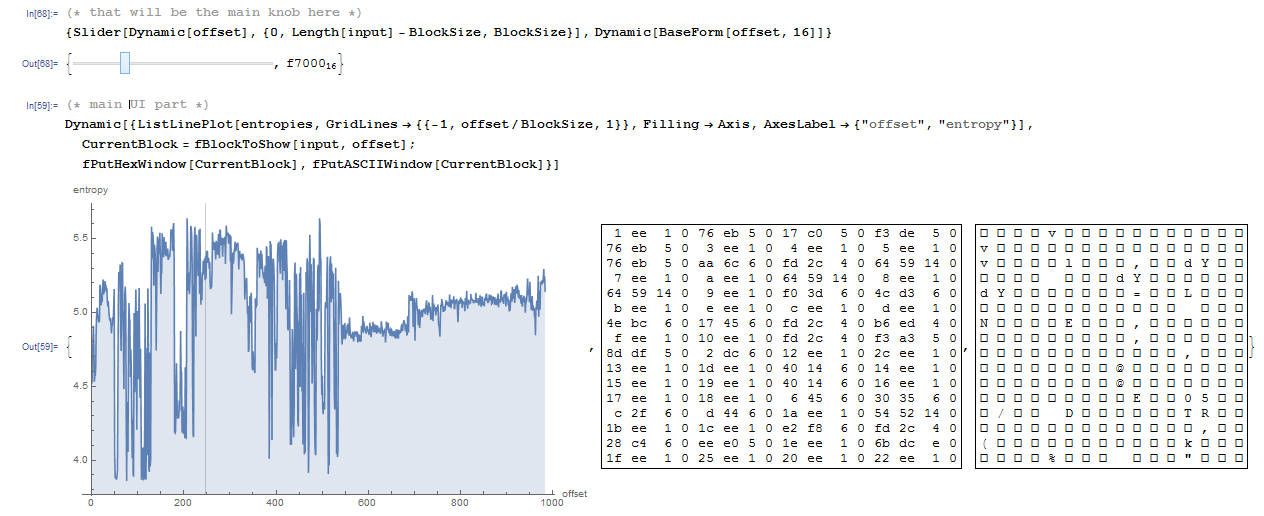
\includegraphics[scale=\FigScale]{ff/entropy/geoipisp1.png}
\end{figure}

There are two parts in graph: first is somewhat chaotic, second is more steady.

0 in horizontal axis in graph mean lowest entropy (the data which can be compressed very tightly, \IT{ordered} in other words) 
and 8 is highest (cannot be compressed at all, \IT{chaotic} or \IT{random} in other words).
Why 0 and 8? 0 mean 0 bits per byte (byte slot is not filled at all) 
and 8 mean 8 bits per byte, i.e., the whole byte slot is filled with the information tightly.

So I put slider to point in the middle of the first block, and I clearly see some array of 32-bit integers.
Now I put slider in the middle of the second block and I see English text:

\begin{figure}[H]
\centering
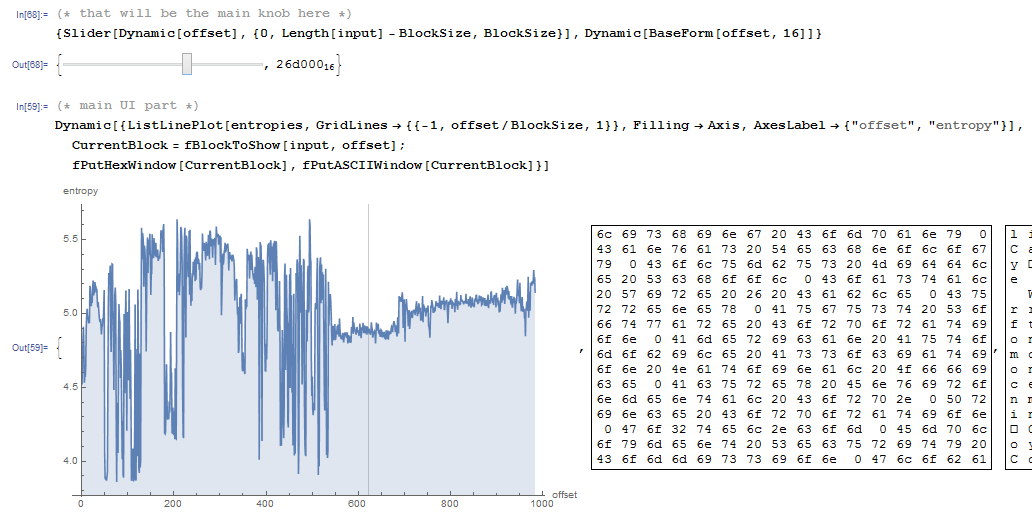
\includegraphics[scale=\FigScale]{ff/entropy/geoipisp2.png}
\end{figure}

Indeed, this are names of ISPs.
So, entropy of English text is 4.5-5.5 bits per byte? Yes, something like this.
Wolfram Mathematica has some well-known English literature corpus embedded, and we can see entropy of Shakespeare's sonnets:

\begin{lstlisting}
In[]:= Entropy[2,ExampleData[{"Text","ShakespearesSonnets"}]]//N
Out[]= 4.42366
\end{lstlisting}

4.4 is close to what we've got (4.7-5.3). 
Of course, classic English literature texts are somewhat different from ISP names and other English texts we can find in binary files 
(debugging/logging/error messages), but this value is close.

\section{TP-Link WR941 firmware}

Now more complex example. I've got firmware for TP-Link WR941 router:

\begin{figure}[H]
\centering
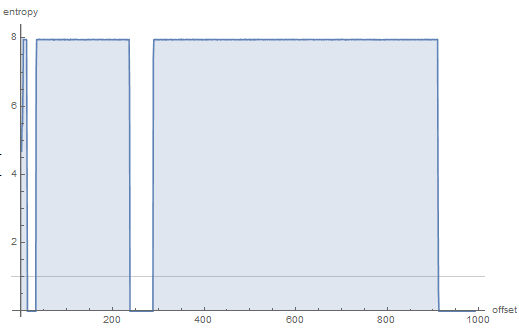
\includegraphics[scale=\FigScale]{ff/entropy/tplink.png}
\end{figure}

Wee see here 3 blocks with empty lacunas.
The first block (started at address 0) is small, second (address somewhere at 0x22000) is bigger and third (address 0x123000) is biggest.
I can't be sure about exact entropy of the first block, but 2nd and 3rd has very high entropy, meaning that these blocks are either
compressed and/or encrypted.

\myindex{Binwalk}
I tried \href{http://binwalk.org/}{binwalk} for this firmware file:

\begin{lstlisting}
DECIMAL       HEXADECIMAL     DESCRIPTION
--------------------------------------------------------------------------------
0             0x0             TP-Link firmware header, firmware version: 0.-15221.3, image version: "", product ID: 0x0, product version: 155254789, kernel load address: 0x0, kernel entry point: 0x-7FFFE000, kernel offset: 4063744, kernel length: 512, rootfs offset: 837431, rootfs length: 1048576, bootloader offset: 2883584, bootloader length: 0
14832         0x39F0          U-Boot version string, "U-Boot 1.1.4 (Jun 27 2014 - 14:56:49)"
14880         0x3A20          CRC32 polynomial table, big endian
16176         0x3F30          uImage header, header size: 64 bytes, header CRC: 0x3AC66E95, created: 2014-06-27 06:56:50, image size: 34587 bytes, Data Address: 0x80010000, Entry Point: 0x80010000, data CRC: 0xDF2DBA0B, OS: Linux, CPU: MIPS, image type: Firmware Image, compression type: lzma, image name: "u-boot image"
16240         0x3F70          LZMA compressed data, properties: 0x5D, dictionary size: 33554432 bytes, uncompressed size: 90000 bytes
131584        0x20200         TP-Link firmware header, firmware version: 0.0.3, image version: "", product ID: 0x0, product version: 155254789, kernel load address: 0x0, kernel entry point: 0x-7FFFE000, kernel offset: 3932160, kernel length: 512, rootfs offset: 837431, rootfs length: 1048576, bootloader offset: 2883584, bootloader length: 0
132096        0x20400         LZMA compressed data, properties: 0x5D, dictionary size: 33554432 bytes, uncompressed size: 2388212 bytes
1180160       0x120200        Squashfs filesystem, little endian, version 4.0, compression:lzma, size: 2548511 bytes, 536 inodes, blocksize: 131072 bytes, created: 2014-06-27 07:06:52
\end{lstlisting}

\myindex{LZMA}
Indeed: there are some stuff at the beginning, but two large LZMA compressed blocks are started at 0x20400 and 0x120200.
These are roughly addresses we have seen in Mathematica.
Oh, and by the way, binwalk can show entropy information as well (-E option):

\begin{lstlisting}
DECIMAL       HEXADECIMAL     ENTROPY
--------------------------------------------------------------------------------
0             0x0             Falling entropy edge (0.419187)
16384         0x4000          Rising entropy edge (0.988639)
51200         0xC800          Falling entropy edge (0.000000)
133120        0x20800         Rising entropy edge (0.987596)
968704        0xEC800         Falling entropy edge (0.508720)
1181696       0x120800        Rising entropy edge (0.989615)
3727360       0x38E000        Falling entropy edge (0.732390)
\end{lstlisting}

Rising edges are corresponding to rising edges of block on our graph.
Falling edges are the points where empty lacunas are started.

I didn't able to force binwalk to generate PNG graphs (due to absence of some Python library), but here is an example how binwalk
can do them: \url{http://binwalk.org/wp-content/uploads/2013/12/lg_dtv.png}.

What can we say about lacunas? By looking in hex editor, we see that these are just filled with 0xFF bytes.
Why developers put them? Perhaps, because they didn't able to calculate precise compressed blocks sizes, so they allocated space
for them with some reserve.

\section{Notepad}

\myindex{Notepad}

Another example is notepad.exe I've picked in Windows 8.1:

\begin{figure}[H]
\centering
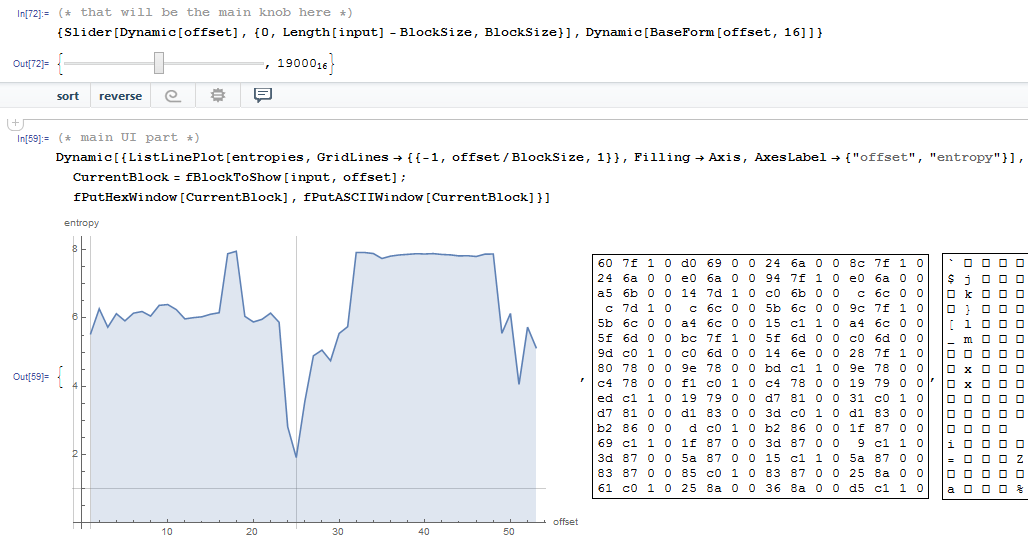
\includegraphics[scale=\FigScale]{ff/entropy/notepad1.png}
\end{figure}

There is cavity at ~0x19000 (absolute file offset).
I opened the executable file in hex editor and found imports table there (which has lower entropy than x86-64 code
in the first half of graph).

There are also high entropy block started at ~0x20000:

\begin{figure}[H]
\centering
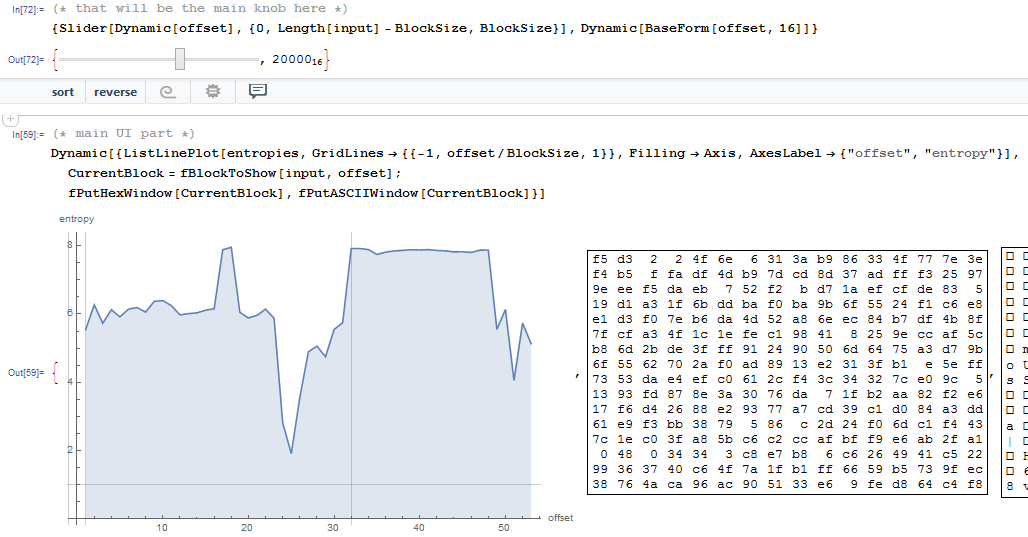
\includegraphics[scale=\FigScale]{ff/entropy/notepad2.png}
\end{figure}

\myindex{PNG}
In hex editor I can see PNG file here, embedded in the PE file resource section (it is a large image of notepad icon).
PNG files are compressed, indeed.

\section{Unnamed dashcam}

Now the most complex example in this article is the firmware of some unnamed dashcam I've received from friend:

\begin{figure}[H]
\centering
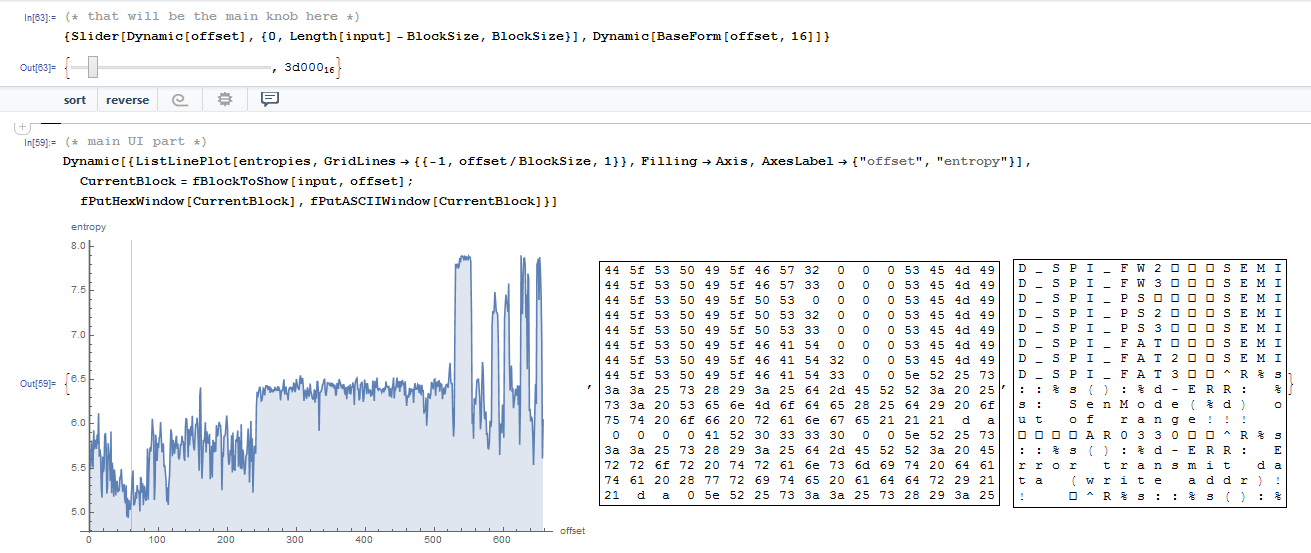
\includegraphics[scale=\FigScale]{ff/entropy/dashcam_text.png}
\end{figure}

The cavity at the very beginning is a English text: debugging messages.
\myindex{MIPS}
I checked various ISAs and I found that 
the first third of the whole file (with the text segment inside) is in fact MIPS (little-endian) code!

For instance, this is very distinctive MIPS function epilogue:

\begin{lstlisting}
ROM:000013B0                 move    $sp, $fp
ROM:000013B4                 lw      $ra, 0x1C($sp)
ROM:000013B8                 lw      $fp, 0x18($sp)
ROM:000013BC                 lw      $s1, 0x14($sp)
ROM:000013C0                 lw      $s0, 0x10($sp)
ROM:000013C4                 jr      $ra
ROM:000013C8                 addiu   $sp, 0x20
\end{lstlisting}

From our graph we can see that MIPS code has entropy of 5-6 bits per byte.
Indeed, I once measured various ISAs entropy and I've got these values:

\begin{itemize}
\item x86: .text section of ntoskrnl.exe file from Windows 2003: 6.6
\item x64: .text section of ntoskrnl.exe file from Windows 7 x64: 6.5
\item ARM (thumb mode), Angry Birds Classic: 7.05
\item ARM (ARM mode) Linux Kernel 3.8.0: 6.03
\item MIPS (little endian), .text section of user32.dll from Windows NT 4: 6.09
\end{itemize}

So the entropy of executable code is higher than of English text, but still can be compressed.

Now the second third is started at 0xF5000. I don't know what this is. I tried different ISAs but without success.
The entropy of the block is looks even steadier than for executable one.
Maybe some kind of data?

\myindex{JPEG}
There is also a spike at ~0x213000. I checked it in hex editor and I found JPEG file there 
(which, of course, compressed)!
I also don't know what is at the end.
Let's try Binwalk for this file:

\begin{lstlisting}
dennis@ubuntu:~/P/entropy$ binwalk FW96650A.bin 

DECIMAL       HEXADECIMAL     DESCRIPTION
--------------------------------------------------------------------------------
167698        0x28F12         Unix path: /15/20/24/25/30/60/120/240fps can be served..
280286        0x446DE         Copyright string: "Copyright (c) 2012 Novatek Microelectronic Corp."
2169199       0x21196F        JPEG image data, JFIF standard 1.01
2300847       0x231BAF        MySQL MISAM compressed data file Version 3

dennis@ubuntu:~/P/entropy$ binwalk -E FW96650A.bin 

WARNING: pyqtgraph not found, visual entropy graphing will be disabled

DECIMAL       HEXADECIMAL     ENTROPY
--------------------------------------------------------------------------------
0             0x0             Falling entropy edge (0.579792)
2170880       0x212000        Rising entropy edge (0.967373)
2267136       0x229800        Falling entropy edge (0.802974)
2426880       0x250800        Falling entropy edge (0.846639)
2490368       0x260000        Falling entropy edge (0.849804)
2560000       0x271000        Rising entropy edge (0.974340)
2574336       0x274800        Rising entropy edge (0.970958)
2588672       0x278000        Falling entropy edge (0.763507)
2592768       0x279000        Rising entropy edge (0.951883)
2596864       0x27A000        Falling entropy edge (0.712814)
2600960       0x27B000        Rising entropy edge (0.968167)
2607104       0x27C800        Rising entropy edge (0.958582)
2609152       0x27D000        Falling entropy edge (0.760989)
2654208       0x288000        Rising entropy edge (0.954127)
2670592       0x28C000        Rising entropy edge (0.967883)
2676736       0x28D800        Rising entropy edge (0.975779)
2684928       0x28F800        Falling entropy edge (0.744369)
\end{lstlisting}

Yes, it found JPEG file and even MySQL data!
But I'm not sure if it's true---I didn't checked it yet.

\myindex{clusterization}
It's also interesting to try clusterization in Mathematica:

\begin{figure}[H]
\centering
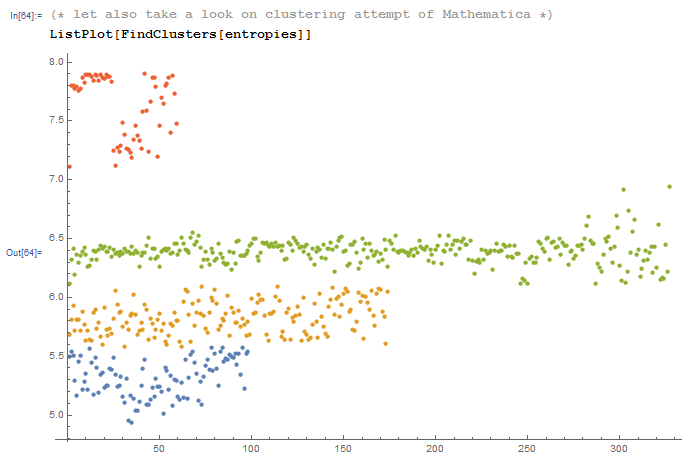
\includegraphics[scale=\FigScale]{ff/entropy/dashcam_clusters.png}
\end{figure}

Here is an example of how Mathematica grouped various entropy values into distinctive groups.
Indeed, there is something credible. Blue dots in range of 5.0-5.5 are probably related to English text.
Yellow dots in 5.5-6 are MIPS code. A lot of green dots in 6.0-6.5 is the unknown second third.
Orange dots close to 8.0 are related to compressed JPEG file.
Other orange dots are probably related to the end of the firmware (unknown to us data).

\section{Conclusion}

Information entropy can be used as a quick-n-dirty method for inspecting unknown binary files.
In particular, it is a very quick way to find compressed/encrypted pieces of data.
Someone say it's possible to find RSA (and other asymmetric cryptographic algorithms) public/private keys 
in executable code (which has high entropy as well), but I didn't tried this by myself.

\section{Links}

Binary files used while writing: \url{http://yurichev.com/blog/entropy/files/}.
Wolfram Mathematica notebook file: \url{http://yurichev.com/blog/entropy/files/binary_file_entropy.nb}
(all cells must be evaluated to start things working).

There is a great (and more complex) online entropy visualizer made by Aldo Cortesi, 
which I tried to mimic: \url{http://binvis.io}.
His articles about entropy visualization are worth reading:
\url{http://corte.si/posts/visualisation/entropy/index.html},
\url{http://corte.si/posts/visualisation/malware/index.html},
\url{http://corte.si/posts/visualisation/binvis/index.html}.

General article about informational entropy in Wikipedia: \url{http://en.wikipedia.org/wiki/Entropy_(information_theory)}.

Handy Linux \IT{ent} utility to measure entropy of a file: \url{http://www.fourmilab.ch/random/}.

\myindex{radare2}
radare2 framework has \IT{\#entropy} command for this.

\section{A word about primitive encryption like XORing}

It's interesting that simple XOR encryption doesn't affect entropy of data.
I've shown this in \IT{Norton Guide} example in the book (\myref{norton_guide}).

Generalizing: encryption by substitution cipher also doesn't affect entropy of data (and XOR can be viewed as substitution cipher).
The reason of that is because entropy calculation algorithm view data on byte-level.
On the other hand, the data encrypted by 2 or 4-byte XOR pattern will result another entropy.

\section{More about entropy of executable code}

It is quickly noticeable that probably biggest source of high-entropy in executable code are relative offsets encoded in opcodes.
For example, these two consequent instructions will produce different relative offsets in their opcodes, 
while they are in fact pointing to the same function:

\begin{lstlisting}
function proc
...
function endp

...

CALL function
...
CALL function
\end{lstlisting}

Ideal executable code compressor would encode information like this:
\IT{there is a CALL to a ``function'' at address X and the same CALL at address Y} without need to encode
address of the \IT{function} twice.

\myindex{UPX}
To deal with this, executable compressors are sometimes able to reduce entropy here.
One example is UPX: \url{http://sourceforge.net/p/upx/code/ci/default/tree/doc/filter.txt}.

\section{Random number generators}

\myindex{GnuPG}
When I run GnuPG to generate new secret key, it asking for some entropy...

\begin{lstlisting}
We need to generate a lot of random bytes. It is a good idea to perform
some other action (type on the keyboard, move the mouse, utilize the
disks) during the prime generation; this gives the random number
generator a better chance to gain enough entropy.

Not enough random bytes available.  Please do some other work to give
the OS a chance to collect more entropy! (Need 169 more bytes)
\end{lstlisting}

This means that good a PRNG produces long high-entropy results, and this is what the secret assimetrical cryptographical key needs.
But \ac{CPRNG} is tricky (because computer is highly deterministic device itself),
so the GnuPG asking for some additional randomness from the user.

Here is my article where I made attempt to calculate entropy of some unknown blocks: \myref{encrypted_DB1}.
